
\documentclass[11pt]{article}

\usepackage{amsmath}
\usepackage[utf8]{inputenc}
\usepackage{geometry}
\geometry{a4paper}
% \geometry{margin=2in} % for example, change the margins to 2 inches all round

\usepackage{graphicx} % support the \includegraphics

\title{TSRT14 --- Lab report update 2}
\author{Group ID: 137}
%\date{} % Activate to display a given date or no date (if empty),
         % otherwise the current date is printed 

\begin{document}
\maketitle
\newpage
\section{Data collection}
The data for this lab was gathered at a scheduled 30-minute session, where the task was to arrange seven microphones in two fundamentally different configurations chosen by the group, and record a sound emitted from a LEGO Mindstorms robot which followed a drawn out path in a stage, in order to localise it. The sound was recorded using a pre-written Matlab script. The first configuration chosen was to evenly space the microphones around the stage as pictured in Figure 1. The second was to evenly space them on just one side of the stage as shown in Figure 2.
\begin{figure}[h!]
\centering
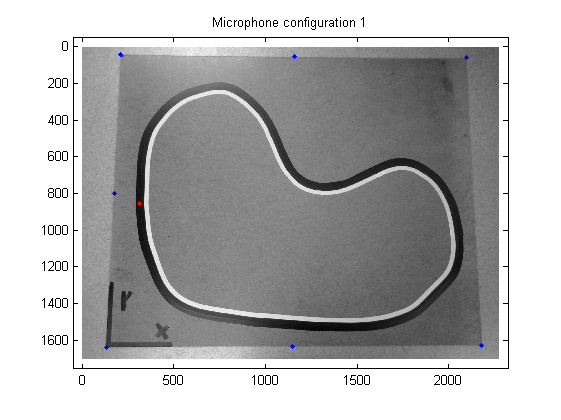
\includegraphics[width=\textwidth]{microphone_configuration_1.png}
\caption{First microphone configuration, believed to be the better one. The start position of the robot is shown in red.}
\end{figure}
\begin{figure}[h!]
\centering
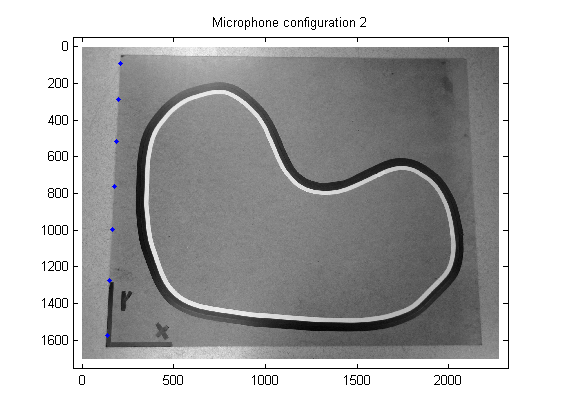
\includegraphics[width=\textwidth]{microphone_configuration_2.png}
\caption{Second microphone configuration, believed to be the worse one. The start position of the robot is shown in red.}
\end{figure}
\newpage
The first was chosen as the configuration believed to be best, since it gathers data in the most even way, so that no "blind spots" would occur. Since this configuration is not always possible in real world examples, an easier configuration was chosen as the second one. These two represent very different approaches to the problem.\\\\
A calibration configuration was also set up, in accordance with the lab PM. Here the microphones were laid out in an arc with the same distance (0.7 meters) to the robot, while the robot emitted its sound at roughly 0.5 second intervals for 45 seconds.
\section{Localisation}
\subsection{Calibration}
The calibration data from the data collection session was used to estimate the spatial error for the localisation. It was calculated by removing the mean of all the microphones for each microphone.


This was then compared to a corresponding normal distribution, as shown for two microphones ($k=2$ and $k=6$) in Figure 3. 
\subsubsection{Conclusion}
The information from the graphs leads to the conclusion that the error $e$ can be assumed to be Gaussian.

\begin{figure}
\begin{center}
  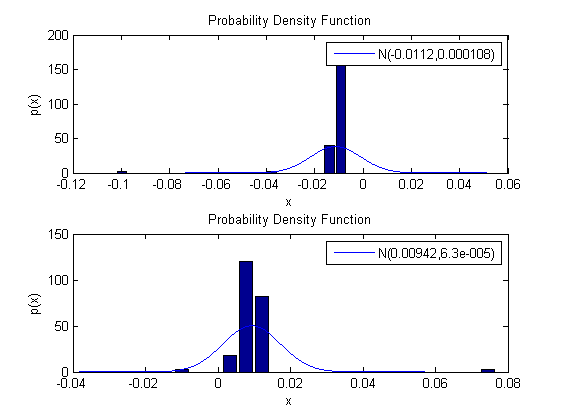
\includegraphics[width=\textwidth]{calibration_ndist_2_and_6.png}
  \caption{Spatial error for two of the microphones, 2 and 6 from the top. The x-axis is in meters.}
  \end{center}
\end{figure}


\subsection{Signal modeling}
The modeling consists of two different TDOA approaches, one with pairwise differences, referred to as TDOA2 in the toolbox, and one with an additional variable $r_0$, which is the unknown distance from the target to each sensor, referred to in the toolbox as  TDOA1.

\[
  y = 
  \begin{bmatrix}
    |th_1 - p| + r_0 \\ 
    |th_2 - p| + r_0 \\ 
    |th_3 - p| + r_0 \\ 
    |th_4 - p| + r_0 \\ 
    |th_5 - p| + r_0 \\ 
    |th_6 - p| + r_0 \\ 
    |th_7 - p| + r_0 \\ 
  \end{bmatrix} + e
\] 



\[
  y = 
  \begin{bmatrix}
    |th_1 - p| - |th_2 - p| \\
    |th_1 - p| - |th_3 - p| \\
    |th_1 - p| - |th_4 - p| \\
    |th_1 - p| - |th_5 - p| \\
    |th_1 - p| - |th_6 - p| \\
    |th_1 - p| - |th_7 - p| \\
    |th_2 - p| - |th_3 - p| \\
    |th_2 - p| - |th_4 - p| \\
    |th_2 - p| - |th_5 - p| \\
    |th_2 - p| - |th_6 - p| \\
    |th_2 - p| - |th_7 - p| \\
    |th_3 - p| - |th_4 - p| \\
    |th_3 - p| - |th_5 - p| \\
    |th_3 - p| - |th_6 - p| \\
    |th_3 - p| - |th_7 - p| \\
    |th_4 - p| - |th_5 - p| \\
    |th_4 - p| - |th_6 - p| \\
    |th_4 - p| - |th_7 - p| \\
    |th_5 - p| - |th_6 - p| \\
    |th_5 - p| - |th_7 - p| \\
    |th_6 - p| - |th_7 - p| \\
  \end{bmatrix} + e
\]

\subsection{Configuration analysis}
In order to determine which of the microphone configurations is better, a configuration analysis is applied. This can be done in two different ways, the first one being Non-linear Least Squares (NLS), the second Cramér-Rao Lower Bound (CRLB). The CRLB approach is used here. The result of this on the first configuration (Figure 1) gives a plot with a clear minimum which indicates a good configuration, shown in Figure 4.\\
\begin{figure}
\begin{center}
  \includegraphics[width=\textwidth]{crlb2_1.png}
  \caption{Cramér-Rao Lower Bound configuration 1.}
  \end{center}
\end{figure}
The result of this on the second configuration (Figure 2) gives a plot (Figure 5) with no distinct minimum which indicates a bad configuration. 
\subsubsection{Conclusion}
This configuration could be a bit better in hindsight, since it's virtually useless as it stands right now. It could be improved  for example by positioning the microphones around a corner.
\begin{figure}
\begin{center}
  \includegraphics[width=\textwidth]{crlb2_2.png}
  \caption{Cramér-Rao Lower Bound configuration 2.}
  \end{center}
\end{figure}


\subsection{Localisation}
The localisation of the robot was done in two different ways, one using a TDOA approach, and one using NLS using Gauss-Newton.

\subsubsection{TDOA}
The "TDOA2" model was used here, with pairwise differences calculated resulting in 21 data sets in order to remove the unknown time of emission of the sound from the robot.\\
Then the position of the target of every time instance can be estimated by using a non-linear least squares solver from the toolbox.


\subsubsection{NLS with Gauss-Newton}
The non-linear least square model with Gauss-Newton is used to estimate the position of the robot, which gives the result shown in figure 6.
\begin{figure}
\begin{center}
  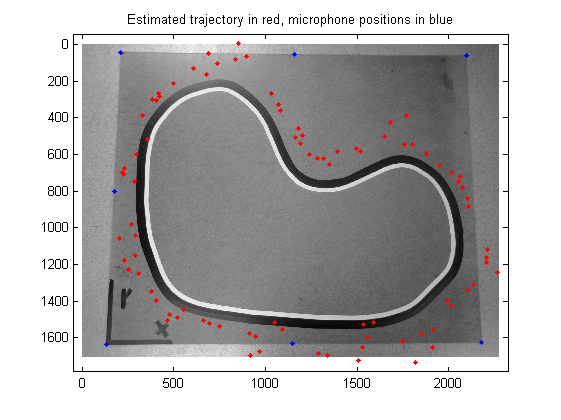
\includegraphics[width=\textwidth]{NLS_Gauss_all_around.png}
  \caption{NLS with Gauss-Newton.}
  \end{center}
\end{figure}

\begin{figure}
\begin{center}
  \includegraphics[width=\textwidth]{TDOA_all_around.png}
  \caption{TDOA2 approach.}
  \end{center}
\end{figure}


\subsubsection{Conclusion}
The different approaches, NLS Gauss and TDOA2, are very close to each other in appearance, which can be observed in Figure 6 and 7.

\subsection{Tracking}
The estimation in the previous task is not the optimal way to estimate the position of the target, since a given position is very much dependent on the previous position. An extended kalman filter can be used to account for this dependence. 

A constant velocity (CV) model and a Coordinated Turn (CT) model was used for this, with TDOA2 as measurement models, the CV model is described in the following way.
\begin{align*}
x = [x, y, v_x, v_y]^T
\end{align*}
\[
  \bar{x}[k+1] = 
  \begin{bmatrix}
    1 & 0 & \frac{\Delta T}{2} & 0 \\
    0 & 1 & 0 & \frac{\Delta T}{2} \\
    0 & 0 & 1 & 0 \\
    0 & 0 & 0 & 1 \\
  \end{bmatrix}
  \bar{x}[k] + \bar{v}
\]

where $\Delta T = 0.5$ s, and $v_x$ and $v_y$ are the velocities of the target. Both of the models were constructed through functions in the toolbox, as $\verb+exnl('cv2d')+$ and $\verb+exnl('ctcv2d')+$ respectively.
The results are shown in plots 7, 8, 9 and 10.\\
\begin{figure}
\begin{center}
  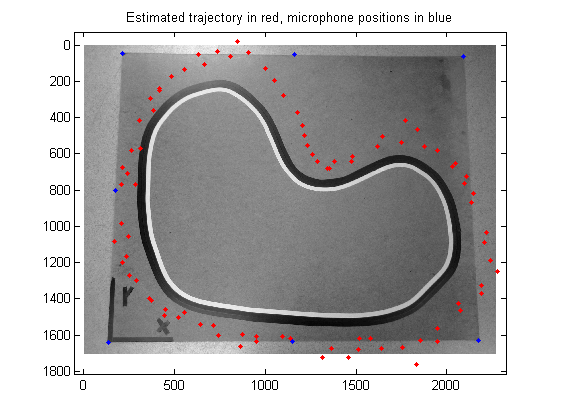
\includegraphics[width=\textwidth]{ekf_CV_TDOA.png}
  \caption{A constant velocity model has been used here, which tracks it quite well except for a slight bias which might have to do with 
the speaker position on the robot.}
  \end{center}
\end{figure}
\begin{figure}
\begin{center}
  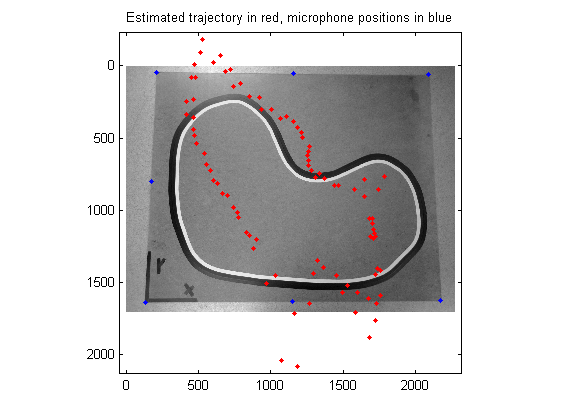
\includegraphics[width=\textwidth]{ekf_CV_TDOA_one_reference.png}
  \caption{A constant velocity model is also used here, but with only one microphone as a reference.}
  \end{center}
\end{figure}
\begin{figure}
\begin{center}
  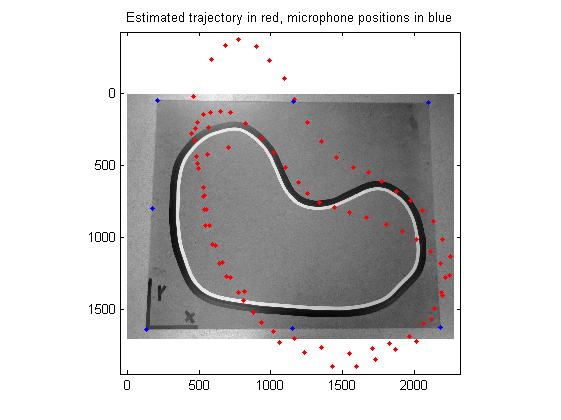
\includegraphics[width=\textwidth]{ekf_CTCV_TDOA.png}
  \caption{This figure shows a coordinated turn model with cartesian velocity (CTCV). It has quite a bit of drift which could be because the track is not suited for this model. A more circular track for example would be better.}
  \end{center}
\end{figure}
\begin{figure}
\begin{center}
  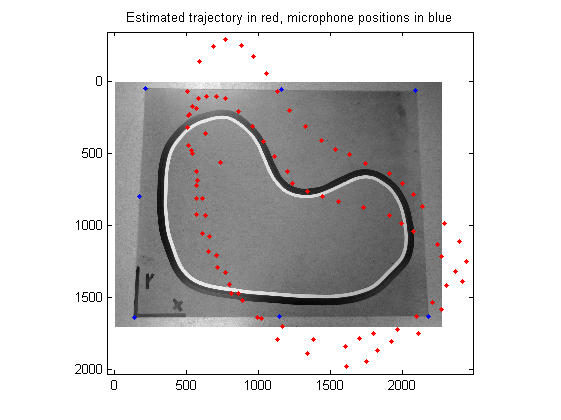
\includegraphics[width=\textwidth]{ekf_CTCV_TDOA_one_reference.png}
  \caption{This is also a CTCV model, but with just one microphone as reference. It's slightly better than the CV model with just one microphone, but not by much.}
  \end{center}
\end{figure}

\subsubsection{Conclusion}
Since the TDOA2 approach with the 21 artificial measurements are linearly dependent, in contrast to the other approach where they are not. This means that there isn't any additional information in the first approach. Alas, they are almost equal in accuracy.


\newpage
\subsection{Sensitivity analysis}
Since the positions of the sensors are measured by hand, the accuracy is probably a bit off. To get a feeling for how the accuracy changes with different stated sensor positions, some of the sensors' positions was changed in the code.
The model used was Constant Velocity with TDOA2. When changing positions in code the differences starts to show at around 5 centimeters, which seems reasonable given the previous variance of errors. Figure 11 and 12 show the CV TDOA2 model with the microphone positions randomly displaced from their initial positions, with a change of 5 and 10 cm respectively.


\begin{figure}
\begin{center}
  \includegraphics[width=\textwidth]{sensitivity_analysis.png}
  \caption{Randomly displaced by 5 centimeters.}
  \end{center}
\end{figure}

\begin{figure}
\begin{center}
  \includegraphics[width=\textwidth]{sensitivity_analysis_0_1.png}
  \caption{Randomly displaced by 10 centimeters.}
  \end{center}
\end{figure}




\end{document}
